\chapter{Experiments}
\label{capitolo5}
\thispagestyle{empty}
If a smartphone Wi-Fi is left turned on it emits a number of probe requests. If also the Bluetooth is turned on, we can stimulate the smartphone to emit some Bluetooth signals. Both the probes and the Bluetooth signals are identify by two different MAC addresses based on the wireless communication that we are using.\\
Pair the Wi-Fi MAC address and the Bluetooth MAC address permits to identify uniquely a mobile device. In fact those two signals derive from the same device but they are not immediately related. As we will see below, the found values are completely different, but they represent the same information: the distance.\\
\linebreak
The distance between the two mobile devices can be expresses in different way:
\begin{itemize}
\item \textbf{Time of arrival (ToA):} the estimation of the distance is obtained by measuring the signal propagation time. (The Time of Flight is \(T_f = \frac{d}{c}\). \(d\) is the distance between the nodes and \(c\) is the speed propagation (c = 299792, 458km/s)) -- questo magari e' evitabile;
\item \textbf{Time Difference of Arrival (TDoA):} in TDoA the receivers deduce the distance from instant differences and propagation speeds;
\item \textbf{Angle of Arrival (AoA):} In AoA there are directional antennas to estimate the signal arrival angle and deduce the distance;
\item \textbf{Received Signal Strength Indicator (RSSI):} RSSI use the signal attenuation to infer the distance, in fact a signal attenuates during propagation.
\end{itemize}
Line-Of-Sight (LOS) propagation is a characteristic of signals propagation which means waves which travel in a direct path from the source to the receiver. In closed environments is difficult to have a straight line between a sender and a receiver. The signal is affected to multipath, that is the propagation of the signal through different path. It is caused by atmospheric ducting, reflection and refraction caused by walls, body, windows, etc... .\\
These issues make inaccurate techniques like ToA, TDoA or AoA. So, in our experiments we choose the RSSI based approach.\\
\linebreak
It is important to remind that we are not only focused on the absolute distance between a sender ad a receiver. We want to determine if the Wi-Fi and the Bluetooth signals have the same path loss to establish if the device is the same.\\
\linebreak  
In this section, are first described the experimental test-bed and the devices used during the experiment. Then the analysis of the device's Wi-Fi and Bluetooth parameters are presented along with discussions and graphics. After the study and the choice of the parameters, the real matching experiment is explained. Successively the coupling algorithms and the methodology are described. In the end there is the interpretation of the results. (ampliare meglio e segnare le sezioni mano a mano che lo scrivo)\\

- dichiarazioni su che esperimenti sono stati fatti\\
\section{Preliminary experiments}
In this experiment we have captured the Wi-Fi probes (containing the Wi-Fi RSSI) and the Bluetooth signals (RSSI, TPL, LQ, echo round trip time).\\
The goals are understand the correlation between distance and the signals originating from the target devices and also understand the relation between Wi-Fi and Bluetooth. In fact, our main scope is not find the absolute position of a device, but comprehend if the Bluetooth and the Wi-Fi signals have origin from the same device. 
\subsubsection{The environment}
The preliminary experiments were held in an home environment with a dimension of 9.50 meters x 4.50 meters and an area of 42.75 m\textsuperscript{2}.
During the first phase of the experiment, the home environment was chosen because it was important to have an isolated environment and no other devices that could cause noise. In addition, it was also crucial to have a direct path between the studied devices.\\
\subsubsection{The devices}
The target devices used in during this experiment were a LG-E450 with Android Kit Kat 4.4.2 (credo) (Ultra Slim custom ROM) and an Ipad ?? with iOs 10. \\
\linebreak
A Raspberry Pi 3 was used to capture Wi-Fi probes and Bluetooth signals. The Wi-Fi module was a NETGEAR W150 and the Bluetooth module was the internal one. The presence of the Raspberry Pi's case does not influence the strength of the signals.
\subsubsection{Execution (o Implementation?)}
The Raspberry Pi were placed in a fixed point, while the target devices were moved in different distances every 10 minutes. The path between the Raspberry Pi and the devices has a straight line without any obstacle in the middle.\\
In the end, our script made the average of all the values to obtain a single value for each position.
\subsection{Results}
As explained before, we want to understand if the collected parameters are in relation with the distance and if they are in relation among each others. It is also important comprehend how we can infer the distance from an RSSI value and study the other variables in order to understand if they are useful in our case.
\subsubsection{Bluetooth}
The Bluetooth signals analyzed during this experiment are the connection based RSSI, the TPL (Transmit Power Level), the LQ (Link Quality), the echo round trip time (obtained from ping) and the RX power level (obtained from inquiry with RSSI).\\
From figure X, the following observations can be made:
\begin{figure}[htbp]
\centering
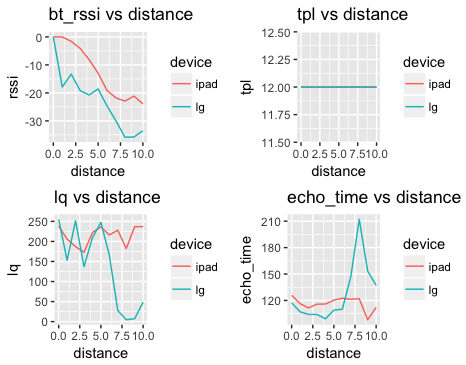
\includegraphics[scale = 0.8, keepaspectratio]{multiple_bt}
\caption{multiple bt}
\end{figure}
\paragraph{Connection based RSSI:} The Received Signal Strength Indicator strongly depends to the distance. It starts from 0 dBm, which means that the target device is inside the GRPR and goes down. As we can note from the image, the iPad chipset is more powerful than the LG one. In fact it's easy to imagine that after ten meters the LG lose the connection (-35 dBm is the maximum for RSSI value), instead the iPad can move apart and be connected yet. So, the RSSI value strongly depends from the device model.\\
Finally, we supposed the curves follows a logarithmic trend as all the decibel values. This is in part true, but not so evident as we imagine. However is evident that is possible to infer the distance starting from RSSI.
\paragraph{LQ:} The link quality, as specification said, start from 255 if the connection is strong and goes down until 0 when the connection is poor. In our experiment the LQ values poorly correlates with the distance. When the devices are near and distant from the Raspberry Pi the value is respectively high and low, but in the middle distance it is not meaningful. For these reasons, for our measurement LQ is discarded.
\paragraph{TPL:} 
Fig. X shows a horizontal straight line for Transmit Power Level values, in fact this value does not change during a Bluetooth connection. The iPad and LG lines are overlapping in 12 dBm. This fact makes impossible use TPL in our calculation.
\paragraph{Echo Round Trip Time:} Echo RTT is obtained pinging the target device. It measures the round-trip time (RTT) for messages sent from the originating host to a destination computer that are echoed back to the source.\\
We have imagined the more is the distance and the more is the round-trip time, but this supposition is not completely true. In fact, the iPad has a RTT of approximately 120ms during all the phases of the experiment; the LG RTT decrease until 4 meters and then rapidly increase. In figure X are shown the trends of the round trip time of echo requests. Also the Echo RTT is discarded.
\paragraph{RX Power Level}
The Raspberry Pi Bluetooth chipset provide absolute RX power level through inquiry, instead of the relative RSSI values as suggested by Bluetooth specification that depends on the GRPR range. Fig. X certainly establishes the RX power level shows a great correlation with distance. Also in this case, there are evident difference between the LG RX power level and the iPad RX.

\begin{figure}[H]
\centering
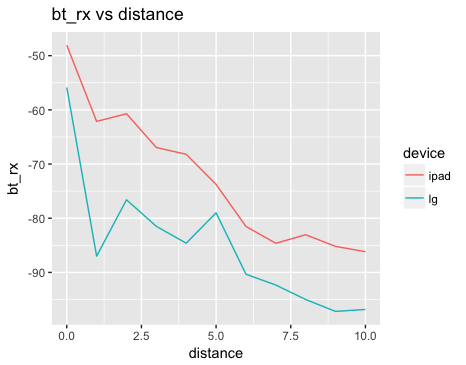
\includegraphics[scale = 0.8, keepaspectratio]{bt_rx_vs_distance}
\caption{bt rx}
\end{figure}

\subsubsection{Bluetooth RSSI vs Bluetooth RX Power Level}
As we have seen before, the two principal Bluetooth signals parameters are the RSSI and the RX Power Level. 
They represent the same value, but the first one includes the presence of the GRPR. \\
In figure Y is shown the relation between the two. Their dependence is linear, so it possible to easily convert the RX power level in RSSI  and vice versa.
\begin{figure}[H]
\centering
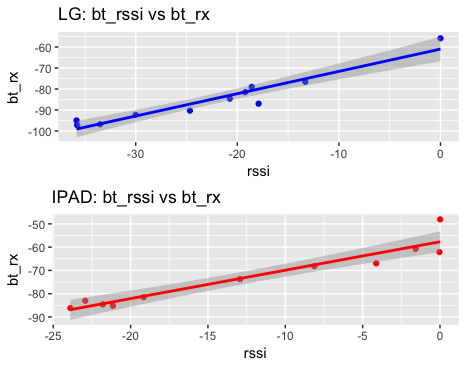
\includegraphics[scale = 0.8, keepaspectratio]{rssivsrx}
\caption{rssi vs rx power level}
\end{figure}
In the following experiments we decide to use only the RSSI. Whilst the RX seems more accurate, the RSSI collects many more values than RX. This permits to be more precise and reduce the time of the experiments thinking also of a real scenario. In fact, as we can see in figure XYZ,  during a ten minutes measurement, the number of RSSI values are almost ten times more than the RX values obtained from the inquiry. The RSSI can be request every seconds (or more), while the RX is affected to the duration of the inquiry that is around 10.24 milliseconds.
\begin{figure}[H]
\centering
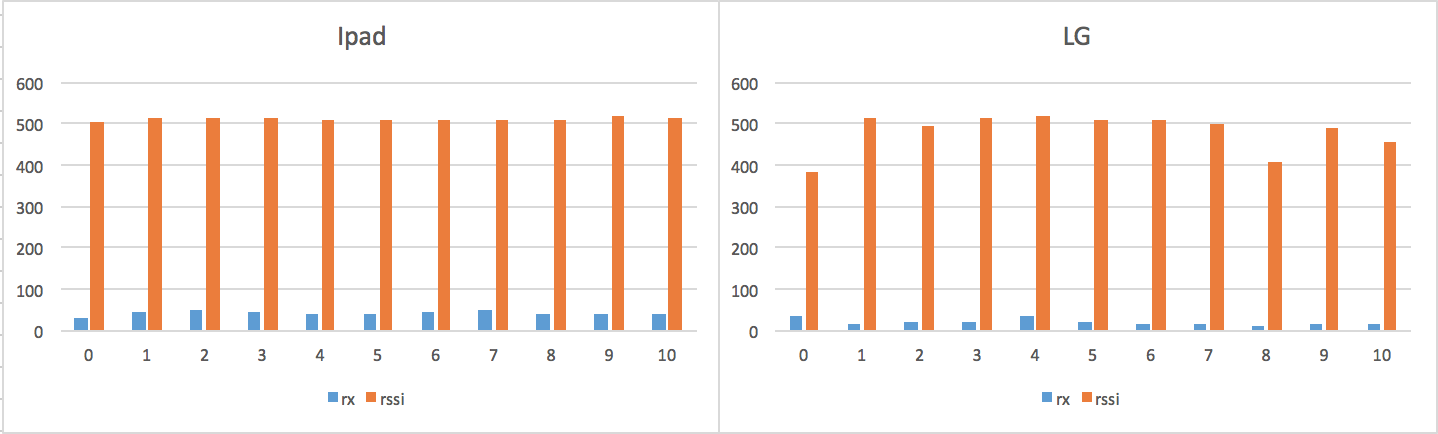
\includegraphics[scale = 0.8, keepaspectratio]{numberofrssirx}
\caption{Number of rssi e rx}
\end{figure}

In addition, the RSSI can be also obtained for non-visible devices, while the RX is only for the visible ones. In a real world scenario, obtain the unseen devices values is a big advantage.



\subsubsection{Wi-Fi}
The last preliminary experiment is the relation between Wi-Fi and distance. As said previously, the Wi-Fi probes have a field containing the RSSI. After capturing it and averaging the data on the basis of the distance, the graphic in figure X was been created.
\begin{figure}[H]
\centering
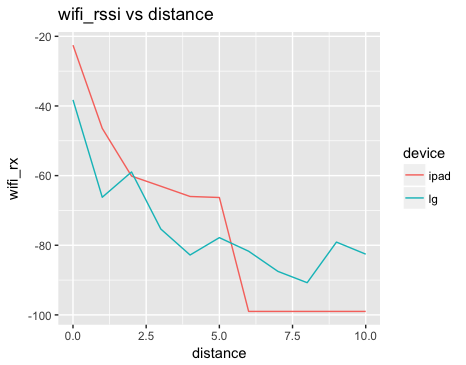
\includegraphics[scale = 0.8, keepaspectratio]{wifi_rssi_vs_distance}
\caption{wifi rssi vs distance}
\end{figure}
The Wi-Fi RSSI follows a logarithmic distribution depending on the distance. It is quite obvious due to the fact that RSSI represents the power of a signal in logarithmic scale. Therefore, as we imagine, the Wi-Fi RSSI is a good indicator of the distance of a device.\\
The distribution of the Wi-Fi RSSI is rather similar to the distribution of the Bluetooth RX power, but the signal strength is higher in Wi-Fi. This is due to the fact that the Wi-Fi range is greater than the one of Bluetooth, which is only around 10 meters for a Class 2 device.


\subsection{Parametri per l'esperimento sala}
In the previous sections, we have analyzed which parameters fit better with the distance. The choices has been Wi-Fi RSSI, Bluetooth RSSI and Bluetooth RX power. As regards Bluetooth was chosen only the RSSI due to the fact its high number of collectible values and the possibility of capturing data also in non-visible mode.\\
Hence, in the following experiment we will only consider Bluetooth RSSI and Wi-Fi RSSI.\\
In the experiment above, we understand that different devices have different RSSI-distance logarithmic curve. This is due to the different internal chipset of the devices. In figure X are shown the different logarithmic trends of five different smartphones and tablets. (Grafico con tutte le curve logaritmiche dei device, uno per bt e l'altro per wifi) piccole considerazioni sui grafici (es. lg e' il piu' scarso, quest'altro e' il piu' forte. i samsung sono simili...)\\
\linebreak
It is also important understand the relation between Wi-Fi and Bluetooth RSSI. It is plotted in the following graph (figure X). The dependence between Wi-Fi and Bluetooth is linear and it is possible to convert the Bluetooth in Wi-Fi and vice versa. Also in this case every device model has a different characteristic curve trend, so a model for each device is created.\\
This relation is fundamental in the matching of Wi-Fi and Bluetooth MAC address.
\section{Esperimento sala}
Starting from the previous data and considerations, now we can explain the real MAC address coupling experiment.\\
\linebreak
During this test we have collected the Bluetooth RSSI and the Wi-Fi probes of 15 devices placed randomly. The devices positions are known, and they are kept in the same position during all the experiment's time. In this way we obtain two different RSSI signals (Bluetooth and Wi-Fi) of each device at the same time. This signals aren't related because they come from two different chipset. The goal is pair two MAC Address, one coming from Wi-Fi and the other one coming from Bluetooth signals, to identify uniquely a device. Pair the Mac Addresses means understand if the Wi-Fi and the Bluetooth RSSI have origin from the same device.\\
\linebreak
In order to couple the two RSSI we create various algorithm and test them to understand which algorithm is better as matching one.

\subsubsection{The environment}
Also this phase was held in an home environment with a dimension of 9.50 meters x 4.50 meters and an area of 42.75 m\textsuperscript{2}.
The home environment was chosen because it was important to have an isolated environment and no other devices that could cause noise and it was also crucial to have a direct path between the devices.\\
In the figure X is shown the planimetry of the room. It is divided in 50 squares of side 0.9 meters and an area of 8.1 m\textsuperscript{2}.\\
\linebreak
An essential alternative is the scenario choice. There are two possibilities: anchor based or anchor free. In the anchor based scenario only the anchor nodes (in our case the Raspberry Pis) knows the position. The other nodes (in our case the devices) derive the position through the anchor. This coordinate system is absolute. In the anchor free scenario no node knows his position. A relative coordinate system is obtained.\\
Our choice was the anchor based scenario, because only the Raspberry Pis are able to catch the probes and manipulate the data. In fact, the target devices are passive.
\subsubsection{The devices}
In the environment we place in a random way five different target devices. Every device is moved in three different random positions in order to simulate the presence of 15 different devices.\\
The used devices are:
\begin{itemize}
\item a Samsung S advance with Android ??? (CyanogenMOD)
\item a LG-E450 with Android Kit Kat 4.4.2 (credo) (Ultra Slim ROM)
\item a Samsung S 3 mini with Adroid 5.??? (CyanogenMOD)
\item an iPad with iOs 10
\item a Samsung Tablet ???
\end{itemize}
As anchors we used 4 Raspberry Pis, with the NETGEAR dongle, in the four corners of the room. In the second phase two more Raspberry Pis were added as in figure X. \\
This configuration permits to cover all the zone of the room and to have different capturing angles.

\subsubsection{Execution (o Implementation?)}
During the experiment the Raspberry Pi stay in a fixed point and the five target devices where placed in three different positions every 10 minutes. \\
At the end of the capturing phase the script deletes the corrupted data and generates a Wi-Fi dataset and a Bluetooth one.\\
The datasets are composed of:
\begin{itemize}
\item a column for each Raspberry Pi (4 or 6 columns, depending on the configuration) containing the RSSI value captured by the respectively Raspberry Pi;
\item a MAC Address column (Wi-Fi or Bluetooth, depending on the dataset) indicating the MAC address device;
\item a timestamp column indicating the time of capture.
\end{itemize}
Each row represents a tuple of values captured in the same instant (same timestamp).
In this way was created a dataset with \textit{n} rows and 6 columns (in case of 4 Raspberry Pis configuration), one for the Wi-Fi and one for the Bluetooth.\\
\linebreak
After this process, we calculate the average of the RSSI of each device for each Raspberry Pi in the two datasets. As a result, we have two different datasets (Bluetooth and Wi-Fi) with 15 lines, one for each device. (In figure X is represented an example of Bluetooth dataset. There are 4 columns with the RSSI and one column with the MAC Address. In the first line there is the BOOOH1 device, its rasp1 RSSI is -666, rasp2 RSSI is -66 and so on. sistemare qua, mettere un immagine con i due dataset separati cosi si capisce un po' meglio.)

\section{Algorithms}
After the capturing phase and the manipulation of the datasets, we focused on the matching algorithms. Various approaches were tested, the best ones are:
\begin{itemize}
\item normalization;
\item RSSI conversion from Bluetooth to Wi-Fi;
\item RSSI conversion from Bluetooth/Wi-Fi to distance;
\item trilateration;
\item fingerprint.
\end{itemize}
In all of these algorithms our goal is pair a line of the Wi-Fi dataset with one of the Bluetooth dataset or vice versa. In fact, each line in the Wi-Fi dataset represents the Wi-Fi signal of a device and we want to find its equivalent in the Bluetooth dataset finding its most similar line.

\paragraph{Euclidean Distance}
In order to find the most similar line we use the euclidean distance. It is the straight-line distance between two, or more, points in euclidean space. In our case, we have 4 points, one for each Raspberry Pi. The euclidean distance is calculated as follows:\\
\(d(w,b) = \sqrt{(w_1 - b_1)^2 + (w_2 - b_2)^2 +... + (w_i - b_i)^2 + ... + (w_n - b_n)^2}\)
where \(w_i\) is the \(i^{th}\) Wi-Fi RSSI and \(b_i\) is  is the \(i^{th}\) Bluetooth RSSI, with \(i = 1, 2, ..., n\) and \(n = 4\) or \( n = 6 \) depending on the configuration.\\
\(d(w,b)\) is close to 0 if the two lines are very similar and became greater if the lines are different.\\
\linebreak
Every time we use an algorithm, at the end of the process, we compare each Wi-Fi line with each Bluetooth line using the euclidean distance. It permits to create for each Wi-Fi address a list of Bluetooth addresses. That is an increasing order list based on the euclidean distance, the value closest to zero is the first of the list, the greatest value is the last one. So, on top of list there are the Bluetooth MAC addresses that are more similar to the Wi-Fi MAC address. Presumably there is his correspondent and then we can match them.

\subsection{Normalization}
The simplest algorithm we have implemented is the normalization of each line.\\
The normalization is a process that adjust values measured on different scales to a common scale, e.g. between 0 and 1.\\
Both the Wi-Fi RSSI and the Bluetooth one represent the strength of the respective signal, but they are on different scales (i.e. the Wi-Fi RSSI is more powerful than the Bluetooth one). Thanks to normalization we can take back these two values on the same 0 and 1 scale.\\
\linebreak
We have normalized separately each line of the two datasets in order to standardize Wi-Fi and Bluetooth data for the same device.\\
The normalization formula is:\\
\( z_i = \frac{x_i-min(x)}{max(x)-min(x)} \)\\
where \( x=(x_1,..., x_n)\) and \(z_i\) is the \(i^{th}\) normalized data.\\
\linebreak
After normalizing the data, we obtain two datasets of values between 0 and 1 representing the Wi-Fi RSSI and the Bluetooth RSSI in a common scale. Now it is possible compare the data and match the device lines.
(immagine dataset normalizzato?)

\subsection{RSSI conversion from Bluetooth to Wi-Fi}
In section 5.X we talked about the linear relation between the Wi-Fi RSSI and the Bluetooth RSSI. This relation was used to convert the Bluetooth values of the Bluetooth dataset in Wi-Fi values. As mentioned above, every device has a different trend, so five different functions were used during the conversion.\\
Thanks to that, we have obtained two Wi-Fi datasets (the real one and the fake one). The last part of the algorithm is to compare each line of the datasets using the euclidean distance and pair the addresses.

\subsection{RSSI conversion from Bluetooth/Wi-Fi to distance}
Starting from the dependence between RSSI (Bluetooth or Wi-Fi) and the distance we elaborated this algorithm. The idea is to convert the RSSI of the two datasets in distance and then, using the euclidean distance, match the line that are more similar between them.\\
\linebreak
In order to convert the RSSI in distance is possible to use the following formula and use the inverse:\\
\(RSSI = p_0 - 10 \alpha log{\frac{d}{d_0}}\)\\
\begin{itemize}
\item \(RSSI\): the RSSI value (path loss);
\item \(p_0\): the received power from the node when the distance is \(d_0\) (RSSI in \(d_0\));
\item \(d\): distance sender-receiver
\item \(\alpha\): a path loss constant. It assumes values between 1 and 3, depending on the environment
\end{itemize}
The distance precision strongly depends on the values that are used in the previous formula. The right calculation of \(\alpha\) and \(p_0\) are fundamental in order to obtain an accurate distance value.\\
\(\alpha\) is determined by the environment in which the devices are located and can be found using the inverse formula of the RSSI. \(p_0\), that is the power level measured at 1 meter, was determined in an empirical way during the previous tests.\\
\linebreak
As we can see, using the formula (X.Y) is quite complicated due to the estimation of the previous parameters. Furthermore, in our case the distance calculation was not so accurate as we could expect.\\
\linebreak
So, in order to convert the RSSI in distance the curves obtained in section 5.XX were used. We create a different curve for each device and for each technology used (Wi-Fi or Bluetooth). It is useful due to the differences of power among the devices.\\
\linebreak
Of course, the choice curve was the logarithmic one (we analyzed the behaviour in the previous sections).\\
We also use a linear model to convert the RSSI to the distance and the results are not so different.

\subsection{Trilateration}
Trilateration is trigonometric approach for tracking mobile objects considering the concept of circles. Since the device knows distance from a minimum of three known Raspberry Pi, trilateration is performed to determine its coordinates. The position is obtained intersecting the circles created by the distance between devices and anchors; the point of intersection is the coordinate of the target device.\\
\linebreak
In our case, we have 4 or more anchors and not always the intersections are in a single point. In this case the problem of trilateration can be approached from an optimisation point of view. We want to find the point X=\(\left(\phi_x, \lambda_x\right)\) that provides us with the best approximation to the actual position P minimizing the error. For this purpose we use the Ordinary Least Squares (OLS) method: \(\frac{\sum { \left[d_i  -dist\left(X,L_i\right)\right] }^2 }{N}\)\\
Where:
\begin{itemize}
\item \(d_i\) is the distance between the anchor and the target device;
\item \(X\) is the coordinate of the device;
\item \(L_i\) is the coordinate of the \(i^{th}\) anchor.
\item \(N\) is the number of anchors.
\end{itemize}
The device coordinates are obtained minimizing the error.\\
\linebreak
(Forse da qua non si capisce un cazzo)\\
The next step is apply the ordinary least square method to the Wi-Fi dataset and the Bluetooth dataset in order to find the coordinates of each device through Wi-Fi and the coordinates through Bluetooth.\\
Finally we compare the two types of coordinates to check the more similar one and pair the MAC address.

\subsection{Fingerprint}
Fingerprint is one of the most popular method for indoor object tracking. Wi-Fi probe requests and Bluetooth signals located in a certain area create an unique \textit{fingerprint}  that is used for the localization.\\
The fingerprinting based positioning systems are carried out in two phases: off-line and on-line.\\
\linebreak
First one is the off-line phase, during this phase the system is calibrated. The first step is divide the location in squared grids. The grid dimension choice is fundamental to obtain a good measurement of the fingerprint. It is useless to use a dense grid because it is hard to locate Wi-Fi and Bluetooth with the accuracy of centimeters; but it is also useless to use a sparse grid because no significant results would be obtained. \\
In our test we choose to divide the room in fifty squares with a side of 0.9 meters and an area of 0.81 m\textsuperscript{2}.\\
\linebreak
The next step is the collection of the fingerprints and the calibration of each cell. The Raspeberry Pis were used in the previous configuration, four anchors in the angles and two anchors in the middle (as figure XXX). As fingerprint target device we used the LG, the Samsung S Advance and the Samsung S3 mini.\\
The devices are placed in the middle of each cell in order to capture the Wi-Fi fingerprint and the Bluetooth fingerprint. At the end of the process, based on the device, the average of each cell of every Raspberry Pi is calculated. The vector (in table XY) obtained of the RSSI values at a cell is called the location fingerprint of that cell. All the vectors create a fingerprint Wi-Fi dataset and a Bluetooth one.  The datasets are 7 columns and 50 rows, one row for each cell.\\
As we can see this operation is very time consuming. This is a great drawback of the fingerprint method.\\
\linebreak
The second part is called the on-line phase. During this phase the previously created datasets are used to determine the cell in which the device is.

divisione in training e test
scelta algoritmi
percentuali di successo nel training

\section{Results}
The problem is the match between a Wi-Fi MAC address and a Bluetooth one. In particular find which Wi-Fi vector is more similar to a Bluetooth vector and vice versa. For this purpose we use the euclidean distance. For each Wi-Fi MAC address we create a ordered list of Bluetooth MAC addresses from the most similar to the most different.\\
This method has allowed us to use a top-k value approach.

\subsection{Top-k value}
For each target MAC address the ordered list of possible MAC addresses is 15 lines long. \\
Top-k approach means that we select the first \(k\) MAC addresses of the ordered list and decide that the correct MAC address is inside that \(k\) values. We don't know exactly what is the correct MAC address, but we have reduced the possible MAC address.\\
\linebreak 
We identify three breakpoints (the k values):
\begin{itemize}
\item Top 1
\item Top 3
\item Top 5
\end{itemize}
A particular case of top-k is when \(k = 1\). This means that we pick the most similar value and decide that value is the correct MAC address.
In top 3 and top 5 we choose the first 3 or 5 MAC addresses as possible MAC address.\\
\linebreak
In figure X are shown how many corrects MAC addresses are inside the \(k\) values. These percentage values are in a 4 Raspberry Pis scenario.
\begin{figure}[H]
\centering
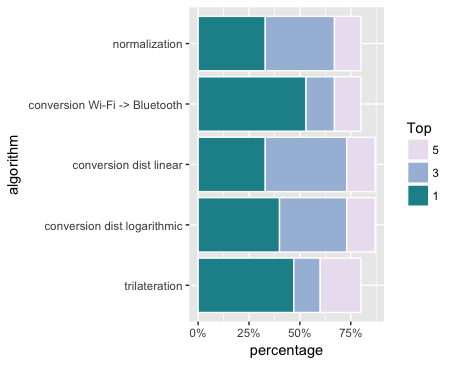
\includegraphics[scale = 0.8, keepaspectratio]{topk_4rasp}
\caption{wifi rssi vs distance}
\end{figure}
As we can see from the figure, the top-5 behavior of the four algorithms is quite similar. The best is the conversion from Wi-Fi/Bluetooth to distance that have a result of 87%.

top k value spiegazione, top k (1, 3, 5) di ogni robo
roc, spiegazione di cos'e' un tp, fp..

\subsection{Top-k values}
grafici tipo a barre con tutti gli algoritmi per i vari top.


\subsection{miglioramento con 6 raspe}
come migliora da 3 a 6


\subsection{True Positive/False Positive rate}
roc

